%% LyX 2.2.1 created this file.  For more info, see http://www.lyx.org/.
%% Do not edit unless you really know what you are doing.
\documentclass[english]{aghdpl}
\usepackage[T1]{fontenc}
\usepackage[utf8]{inputenc}
\setcounter{secnumdepth}{3}
\setcounter{tocdepth}{3}
\usepackage{babel}
\usepackage{verbatim}
\usepackage{float}
\usepackage{mathtools}
\usepackage{amsmath}
\usepackage{graphicx}
\usepackage[unicode=true,pdfusetitle,
 bookmarks=true,bookmarksnumbered=true,bookmarksopen=true,bookmarksopenlevel=3,
 breaklinks=false,pdfborder={0 0 1},backref=false,colorlinks=false]
 {hyperref}
\usepackage{breakurl}

\makeatletter

%%%%%%%%%%%%%%%%%%%%%%%%%%%%%% LyX specific LaTeX commands.

\newcommand*\LyXZeroWidthSpace{\hspace{0pt}}
%% Because html converters don't know tabularnewline
\providecommand{\tabularnewline}{\\}

%%%%%%%%%%%%%%%%%%%%%%%%%%%%%% User specified LaTeX commands.
\usepackage{polski}




\usepackage{amsfonts}
\usepackage{amsthm}


\usepackage[
style=numeric,
sorting=none,
language=autobib,
autolang=other,
urldate=iso8601,
backref=false,
isbn=true,
url=false,
maxbibnames=3,
backend=bibtex8,
]{biblatex}
\usepackage{csquotes}
\DeclareQuoteAlias{croatian}{polish} 


\addbibresource{bibliografia.bib}

\AtBeginDocument{

}

\author{SIMENS Healthkare}
\shortauthor{SIMENS}
\titlePL{DADM project documentation - draft}
\titleEN{}
\shorttitlePL{DADM project documentation}
\shorttitleEN{DADM project documentation}
\thesistype{}
\supervisor{PhD. Tomasz Pięciak}
\degreeprogramme{Biomedical engineering}
\date{2017}
\department{Department of  Automatics and Biomedical Engineering}
\faculty{AGH University of Science and Technology\protect\\[-2mm]
Faculty of Electrical Engineering, Automatics,\protect\\[-2mm] Computer Science and Biomedical Engineering}
\acknowledgements{}
\setlength{\cftsecnumwidth}{10mm}







\makeatother

\begin{document}
\titlepages

\fancypagestyle{plain} { \fancyhf{} \global\long\def\headrulewidth{0pt}
 \global\long\def\footrulewidth{0pt}
 }

\setcounter{tocdepth}{2}

\tableofcontents{}

\clearpage{}

\chapter{List of changes}

\begin{tabular}{|c|c|c|}
\hline 
Name  & Date  & Details\tabularnewline
\hline 
\hline 
Sylwia Mól  & 19-Nov-2017  & Document created\tabularnewline
\hline 
Sylwia Mól  & 20-Nov-2017  & Structure changed\tabularnewline
\hline 
Sylwia Mól  & 21-Nov-2017  & Chapter \textquotedbl{}Authors\textquotedbl{} added, in-out table
added\tabularnewline
\hline 
Malwina Molendowska  & 26-Nov-2017  & Description of 1st module added\tabularnewline
\hline 
Eliza Kowalczyk  & 27-Nov-2017  & Description of 9th module added\tabularnewline
\hline 
Karolina Gajewska  & 27-Nov-2017  & Description of 10th module added\tabularnewline
\hline 
Eliza Kowalczyk  & 28-Nov-2017  & Description of 9th module changed\tabularnewline
\hline
Alicja Martinek  & 28-Nov-2017  & Description of 5th module changed\tabularnewline
\hline 
Mateusz Pabian  & 29-Nov-2017  & Description of 6th module changed\tabularnewline
\hline
Jacek Fidos  & 29-Nov-2017  & Tools description added\tabularnewline
\hline
Anna Grzywa  & 29-Nov-2017  & Description of 8th module added\tabularnewline
\hline 
Magdalena Rychlik & 29-Nov-2017 & Description of 4th module \tabularnewline
\hline 
Magdalena Kucharska & 29-Nov-2017 & Description of 9th module added\tabularnewline
\hline 
 &  & \tabularnewline
\hline 
\end{tabular}

\chapter{Assumptions}

about the app - the aim, what you can do here etc.

\chapter{Structure}

dependences (tree), modules` descriptions \\
 %
\begin{tabular}{|c|c|c|c|}

\hline 
Module  & Input  & Output  & Before that module\tabularnewline
\hline 
\hline 
1 & \textbf{k}-space signals  &  \textbf{x}-space fully reconstructed data  & ——–\tabularnewline
\hline 
2 &  &  & \tabularnewline
\hline 
3  &  &  & \tabularnewline
\hline 
4 & reconstructed, normalized image & Rician noise-free image & intensity correction \tabularnewline
\hline 
5 & reconstructed, normalized image & Rician noise-free image & reconstruction \tabularnewline
\hline 
6 & reconstructed, normalized image; gradient-sequence vectors & estimated diffusion tensor 3D 6-channel image & modules 1-5, 8*
\tabularnewline
\hline 
8 & image & image without non-brain tissues & \tabularnewline
\hline 
9 & image without non-brain tissues & segmentated image & \tabularnewline
\hline 
9 & 320x240 image  & 640x480 image  & denoised data \tabularnewline
\hline 
10  & 1)segmentated image 2)defined plane, image  & 1)3D model (e.g. vtkPolyData) 2)cross-section image  & 1)segmentation 2) denoised data\tabularnewline
\hline 
11 &  &  & \tabularnewline
\hline 
\end{tabular}

\chapter{User guide}

\section{Requirements}

what user need to use this app - e.g. windows version etc

\section{Instruction}

instructions for user - GUI screens etc 

\chapter{Detailed description}

\section{Module 1}

The aim of this module is to formulate mathematical algorithm, which
enables proper data reconstruction for images obtained with parallel
MRI scans. The reconstruction is performed with use of Sensitivity
Encoding (SENSE) algorithm in least squares (LS) solution context
and Tikhonov regularization method.

Generally, parallel MRI acquisitions are targeted to diminish time
needed for data sampling. The usage of multiple coils enabled simultaneous
acquisition of signals. A further step, which is acquiring partial
data from \textbf{k}-space, leads to craved time savings, meanwhile
maintaining full spatial resolution as well as contrast at the same
time. However, the approach of omitting lines in acquisition step
results in data aliasing, i.e. folded images that need further data
processing.

To clearly mark out how data is processed in this module, we list
following reconstruction steps: i) the application of 2D Fourier Transform
transform (2D FFT) to \textbf{k}-space data (acquired raw signals)
from multiple coils. The result is a set of \textbf{x}-space images
with folded pixels, ii) the sensitivity maps estimation of coils profiles
(the information is needed to properly unfold subsampled data) and
iii) the proper unfolding data process with usage of SENSE reconstruction
algorithm and its alterations.

The most crucial step in processing is estimation of sensitivity coil
profiles as a successful image reconstruction with use of pMRI algorithms
highly depends on accurate sensitivity coil assessment. As sensitivity
information varies from scan to scan it is impossible to obtain absolute
maps. To obtain reliable knowledge, reference scans have to be conducted
each time an examination is performed. These low-resolution information
helps to estimate coil profiles with use of the many methods i.e.
dividing each component coil image by a 'sum of squares' image.

It basic formulation, SENSE algorithm is applied to Cartesian MRI
data undersampled uniformly by a factor $r$~(i.e. $r=2$ means that
every other line in \textbf{k}-space is skipped). After Fourier transformation,
each pixel in \textbf{x}-space image received in \textit{l}-th coil
can be seen as weighted sum of $r$ pixels from full FOV, each multiplied
by corresponding localized values of maps. The distance between those
'aliased' points in the full FOV is always equal to the desired FOVy
value divided by subsampling rate. Obviously, depending on subsampling
rate the number of folded pixels changes. Basically, the signal in
one pixel at a certain location $(x,y)$ received from $l$-th component
coil image $D_{l}^{S}$ with chosen subsampling rate $r$ can be written
as: 
\begin{equation}
D_{l}^{S}(x,y)=S_{l}(x,y_{1})D^{R}(x,y_{1})+S_{l}(x,y_{2})D^{R}(x,y_{2})+...+S_{l}(x,y_{r})D^{R}(x,y_{r}),\label{Eq:wzor1}
\end{equation}
where index $l$ counts from 1 to $L$ (number of coils) and index
$i$ counts from 1 to $r$. Eq.(\ref{Eq:wzor1}) can be rewritten
as:

\begin{equation}
D_{l}^{S}(x,y)=\sum_{i=1}^{r}S_{l}(x,y_{i})D^{R}(x,y_{i})\quad\text{for}\quad l=1,...,L.\label{Eq:wzor2}
\end{equation}

Including all $L$ coils the above equation can be rewritten in a
matrix form:

\begin{equation}
\textbf{D}^{S}(\textbf{x})=\textbf{S}(\textbf{x})\textbf{D}^{R}(\textbf{x}),\label{Eq:wzor3}
\end{equation}

The vector $\textbf{D}^{S}(\textbf{x})$ denotes the aliased coil
image values at a specific location \textbf{x} = $(x,y_{i})$ and
has a length of $L$, $\textbf{S}(\textbf{x})$ is a $L$x$R$ matrix
and represents the sensitivities values for each coil at the $r$~superimposed
positions and $\textbf{D}^{R}(\textbf{x})$ lists the $r$ pixels
from full FOV image to be reconstructed. The closed-form solution
of the problem is as follows: 
\begin{equation}
\widehat{\textbf{D}^{R}(\textbf{x})}=(\textbf{S}^{H}(\textbf{x})\textbf{S}(\textbf{x}))^{-1}\textbf{S}^{H}(\textbf{x})\textbf{D}^{S}(\textbf{x}),\label{Eq:wzor4}
\end{equation}
where $\widehat{\textbf{D}^{R}(\textbf{x})}=[\widehat{D^{R}(x,y_{1})},...,\widehat{D^{R}(x,y_{r})}]^{T}$
and $\textbf{S}^{H}(\textbf{x})$ is the conjugate transpose of the
$\textbf{S}(\textbf{x})$ matrix. The final reconstruction image is
defined as: 
\begin{equation}
M(\textbf{x})=\left|\widehat{\textbf{D}^{R}(\textbf{x})}\right|.\label{Eq:wzor5}
\end{equation}

The `unfolding' process can be performed as long as inversion of $\textbf{S}(\textbf{x})$
matrix is possible. Therefore, we cannot set the value of subsampling
rate exceeding the number of coils $L$. To restore full FOV data,
SENSE algorithm has to be recalled for each pixel in aliased \textbf{x}–space
image.

A regularization approach is defined as an~inversion method that
introduces additional information in order to stabilize the solution.
This method is beneficial as it roughly matches the desired solution
and is less sensitive to perturbations of the data. Tikhonov regularization
is a common approach to obtain an inexact solution to a~linear system
of equations. In particular, the Tikhonov regularized estimate reads
as follows:

\begin{equation}
\widehat{\textbf{D}_{reg}^{R}}=\text{arg}\underset{\textbf{D}^{R}}{\text{min}}\left\{ \left\Vert \textbf{D}^{S}-\textbf{S}\textbf{D}^{R}\right\Vert ^{2}+\lambda^{2}\left\Vert \textbf{A}(\textbf{D}^{R}-\textbf{D})\right\Vert ^{2}\right\} ,\label{Eq:wzor6}
\end{equation}

where $\lambda$ is a regularization parameter ($\lambda>0$) and
$\textbf{D}$ is a~prior image known as a regularization image. Selection
of the parameter $\lambda$ and $\textbf{D}$ can be performed using
different procedures. In this module $\textbf{A}$~is assumed to
be an identity matrix. The first term provides fidelity to the data
and the second introduces prior knowledge (e.x. median filtered initial
guess of LS SENSE) about the expected behaviour of $\textbf{D}^{R}$.
The Tikhonov regularization problem is given by:

\begin{equation}
\widehat{\textbf{D}_{reg}^{R}}=\textbf{D}+(\textbf{S}^{H}\textbf{S}+\lambda\textbf{A}^{H}\textbf{A})^{-1}\textbf{S}^{H}(\textbf{D}^{S}-\textbf{S}\textbf{D}).\label{Eq:wzor7}
\end{equation}

A reasonable value for $\lambda$~can be picked using many technique,
i.e. the L-curve criterion or generalized cross-validation.

\textbf{\emph{Module input}}: Synthetic MR images are brain MRI slices
coming from BrainWeb are normalized to {[}0-255{]} (all with intensity
non-uniformity INU=0). Only T1- and T2-weighted data is used. The
dataset is free of noise and the background areas are set to zero.
The slice thickness equals 1 mm. These images are used then to simulate
synthetic noisy accelerated parallel Cartesian SENSE MRI data according
to following steps (the data simulation is performed with use of eight
receiver coils ($L=8$)): i) simulated sensitivity maps (divided into
the ratio 3:1 for real and imaginary parts, respectively) are added
to fully-sampled \textbf{x}-space data, ii) correlated complex Gaussian
noise with different values of standard deviations is added to each
coil image, iii) 2D FFT and data subsampling with chosen reduction
factor $r$ is performed and iv) 2D iFFT is applied to recover data
in \textbf{x}-space. Then, data reconstruction process is conducted.

\textbf{\emph{Module output}}: The output is full resolution reconstructed
data performed with two different algorithms: SENSE (LSE) and Tikhonov
regularization. \\


\section{Module 2}

The Intensity inhomogeneity of the same tissue varies with the location of the tissue within the image. In other words it refers to the slow, nonanatomic intensity variations of the same tissue over the image domain. It can be due to imaging instrumentation (such as radio-frequency nonuniformity, static field inhomogeneity, etc.) or the patient movement. This artifact is particularly severe in MR images captured by surface coils.  Although intensity inhomogeneity is usually hardly noticeable to a human observer, many medical image analysis methods, such as segmentation and registration, are highly sensitive to the spurious variations of image intensities.

The aim of this module is correction of intensity inhomogeneity in MR image using gradient based, surface fitting method. The methods fit a parametric surface to a set of image features that contain information on intensity inhomogeneity. The resulting surface, which is usually polynomial or spline based, represents the multiplicative inhomogeneity field that is used to correct the input image.


\section{Module 3}

Magnetic Resonance Imaging (MRI) is known to be affected by several sources of quality deterioration, due to limitations in the hardware, scanning times, movement of patients, or even the motion of molecules in the scanning subject. Among them, noise is one source of degradation that affects acquisitions. The presence of noise over the acquired MR signal is a problem that affects not only the visual quality of the images, but also may interfere with further processing techniques such as registration or tensor estimation in Diffusion Tensor MRI.

The aim of this module is to estimate the spatial dependent pattern of the variance of noise in SENSE reconstructed images. For this to work some additional information must be known beforehand, such as the sensitivity maps of each receiver coil. In the background of a SENSE MR image, where the SNR is zero, the Rician PDF (Probability density function) simplifies to a (non-stationary) Rayleigh distribution, whose second order moment is defined as:

\begin{equation}
\begin{aligned}
E\left \{ M^{2}\left ( x \right ) \right \}= 2\cdot \sigma_R^{2}\cdot \left ( x \right )
\end{aligned}
\end{equation}

Since $\sigma_R^{2}$ is \textit{x}-dependent, $E\left \{ M^{2}\left ( x \right ) \right \}$ will also show a different value for each \textit{x} position.

Let us assume that each coil in the \textit{x} -space is initially corrupted with uncorrelated Gaussian noise with the same variance $\sigma_n^{2}$ and there
is a correlation between coils $\rho$ so that matrix $\sigma$ becomes:

\begin{equation}
\begin{aligned}
\Sigma= \sigma_n^{2}\begin{pmatrix}
1 & \rho & \cdots & \rho \\ 
\rho & 1 & \cdots & \rho \\ 
\vdots & \vdots & \ddots & \vdots \\ 
\rho & \rho & \cdots & 1
\end{pmatrix}= \sigma_n^{2}\left ( I+\rho\left [ 1-I \right ] \right )
\end{aligned}
\end{equation}
with \textit{I} the $L\times L$ identity matrix and \textit{1} a $L\times L$ matrix of 1's. For each \textit{x} value, we define the global map

\begin{equation}
\begin{aligned}
G_{w_i}=W_i^{*}\left ( I-\rho\left [ 1-I \right ] \right )W_i, \quad i=1,\cdots ,r
\end{aligned}
\end{equation}

Global map $G_w(x)$ can be easily inferred from $G_{w_i}$ values. Note that $G_w(x)$ is strongly related fo the g-factor, so the first equation becomes

\begin{equation}
\begin{aligned}
E\left \{ M^{2}\left ( x \right ) \right \}= 2\cdot \sigma_n^{2}G_w \left ( x \right )
\end{aligned}
\end{equation}

and

\begin{equation}
\begin{aligned}
\sigma_n^{2}=\frac{E\left \{ M^{2}\left ( x \right ) \right \}}{2G_w \left ( x \right )}
\end{aligned}
\end{equation}

By using this regularization we can assure a single $\sigma_n^{2}$ value for all the points in the image. We can now define a noise estimator based on the local sample estimation of the second order moment:

\begin{equation}
\begin{aligned}
\left \langle M^2(x) \right \rangle_x= \frac{1}{\left | \eta(x) \right |}\sum_{p \in \eta(x)}M^2(p)
\end{aligned}
\end{equation}
with $\eta(x)$ a neighborhood centered in x. $\left \langle M^2(x) \right \rangle_x$ is know to follow a Gamma distribution whose mode is $\sigma_n^{2}(\left | \eta(x) \right |-1)/\left | \eta(x) \right |$. Then

\begin{equation}
\begin{aligned}
mode\left \{ \frac{\left \langle M_L^2 \right \rangle_x}{G_w(x)} \right \}=2\sigma_n^2\frac{\left | \eta(x) \right |-1}{\left | \eta(x) \right |}\approx 2\sigma_n^2
\end{aligned}
\end{equation}
when $\left | \eta(x) \right |\gg 1$. The estimator is the defined as

\begin{equation}
\begin{aligned}
\widehat{\sigma_n^2}=\frac{1}{2}mode\left \{ \frac{\left \langle M_L^2(x) \right \rangle_x}{G_w(x)} \right \}
\end{aligned}
\end{equation}
and consequently the noise in each pixel is estimated as

\begin{equation}
\begin{aligned}
\widehat{\sigma_R^2}=\frac{1}{2}mode\left \{ \frac{\left \langle M_L^2(x) \right \rangle_x}{G_w(x)} \right \}G_w(x)
\end{aligned}
\end{equation}

This estimator is only vaild over the background pixels. However, no segmentation of these pixels is needed: the use of the mode allows us to work with the whole image. On the other hand, to carry out the estimation, the sensitivity map of each coil and the correlation between coils must be known beforhand. These parameters are needed for the SENSE encoding, and thus, they can be easily obtained.



\section{Module 4}

The aim of this module is to remove Rician noise from MR images. If both real and imaginary parts of signal are corrupted with zero-mean uncorrelated Gaussian noise with equal variance, the envelope of magnitude signal will follow a Rician distribution. Many processes allow to remove noise, here the method is used to denoise MR images is the linear minimum square error estimator (LMMSE). The main purpose of LMMSE is to find a closed-form estimator for a signal that follows a Rician distributions. It is more efficient than optimization-based solutions. The estimator uses information of the sample distribution of local statistics of the image such as the local mean, the local variance and the local mean square value. In this method, the true value for each noisy pixel is estimated by a set of pixels selected from a local neighborhood. 

The LMMSE estimator for a 2-D signal with Rician distribution is defined: 

\begin{equation}
\begin{aligned}
\widehat{A_{ij}^2} = E\{A_{ij}^2\} + C_{A_{ij}^2M_{ij}^2}C_{M_{ij}^2M_{ij}^2}^{-1}(M_{ij}^2 - E\{M_{ij}^2\} )
\end{aligned}
\label{m4eq1}
\end{equation}
where $A_{ij}$ is the unknown intensity value in pixel $ij$, $M_ij$ the observation vector, $C_{A_{ij}^2M_{ij}^2}$ the cross-covarience vector and $C_{M_{ij}^2M_{ij}^2}$ the covarience matrix. If the estimator is simplified to be pointwise, vectors and matrics become scalar values. Then the assuming local ergodicity with a square nighbourhood around the pixel $ij$, the finally equation for LMMSE is defined: 
\begin{equation}
\begin{aligned}
\widehat{A_{ij}^2} = \langle M_ij^2 \rangle - 2\sigma_n^2 + K_{ij}  (M_{ij}^2 - \langle M_{ij}^2\rangle )
\end{aligned}
\label{m4eq2}
\end{equation} 
with $K_{ij}$
\begin{equation}
\begin{aligned}
K_{ij}^2 =1 - \frac{ 4\sigma_n^2( \langle M_ij^2 \rangle - 2\sigma_n^2)}{\langle M_ij^4 \rangle - {\langle M_ij^2 \rangle}^2}
\end{aligned}
\label{m4eq3}
\end{equation}

The LMMSE estimator is related to the quality of the estimate of the noise variance $\sigma_n^2$. For the noise estimation the mode of the sample mean is used:

\begin{equation}
\begin{aligned}
\widehat{\sigma_n}=\sqrt{\frac{2}{\pi}}mode(\widehat{\mu_1}_{ij})
\end{aligned}
\label{m4eq4}
\end{equation}
 where $\widehat{\mu_1}_{ij}$
\begin{equation}
\begin{aligned}
\widehat{\mu_1}_{ij} = \frac{1}{|\eta_{ij}}\sum_{p\colon\eta_{ij}} I_p
\end{aligned}
\label{m4eq5}
\end{equation}

The use of the LMMSE method should makes the filtering process computationally far more efficient and easier to implement. Also the use of local statistics should decrease estimator dependent of parameters such as the size of window.

\emph{\textbf{Module input}}: Reconstructed, normalized and corrected data.

\emph{\textbf{Module output}}: Image without Rician noise.

\section{Module 5}
Magnetic Resonance images are endangered of being corrupted by noise and artifacts. Since they are used as a basis for medical diagnosis their quality has to be at highest possible level. Noise can be dealt with by changing the parameters of images acquisition, however it increases the scanning time, which is undesirable in medical imaging. To overcome this obstacle, post-processing methods like filtering are employed for denoising. In domain of MRI denoising many filters may be used, though here emphasis is put on Unbiased Non-Local Means (UNLM) filter, which is an extension of NLM filter. In order to understand Unbiased version of this algorithm, the basic one has to be presented.

Having image \textit{Y}, the NLM algorithm calculates the new value of point \textit{p} accordingly to the equation:

\begin{equation}
\begin{aligned}
NLM(Y(p)) = \sum_{\forall q \in Y}^{}w(p,q)Y(q) \\
0 \le w(p,q) \le 1 , 
\sum_{\forall q \in Y}^{}w(p,q) = 1
\end{aligned}
\label{m5e1}
\end{equation}

It can be seen that value of \textit{p} is calculated as weighted average of pixels in the image (\textit{q}), having fulfilled restrictions from \ref{m5e1}. To determine before mentioned average the similarity between squared neighbourhoods widows centered around pixels \textit{p} and \textit{q} are calculated. The size of the window can determined by the user, defined by parameter $R_{sim}$. Equation \ref{m5e2} shows how to determine this similarity.

\begin{equation}
w(p,q) = \frac{1}{Z(p)}e^{\dfrac{d(p,q)}{h^2}}
\label{m5e2}
\end{equation}

\textit{Z(p)} is the normalizing constant which also uses exponential decay parameter \textit{h} and the weighted Euclidean distance measure for pixels in each neighbourhood, called \textit{d}.

\begin{equation}
Z(p) = \sum_{\forall q}^{} e^{\dfrac{d(p,q)}{h^2}}
\label{m5e5}
\end{equation}

\begin{equation}
d(p,q) = G_{p}||Y(N_{p}) - Y(N_{q})||^{2}_{R_{sim}}
\label{m5e6}
\end{equation}

In above equation $G_p$ stands for a Gaussian weighting function that has a 0 mean and standard deviation usually equal to 1.

Once NLM filter is fully explained, unbiased extension of it can be examined. It builds on the properties of MRI signal. According to \cite{5a1} the magnitude signal of MRI follows a Rician distribution. Furthermore, for low intensity regions the Rician distribution approaches to a Rayleigh one, whilst for high intensity it shifts towards Gaussian. It was investigated that this bias can be handled by filtering the squared MRI image, since it is not longer signal-dependent \cite{5a1}. As a consequence the bias, which equals 2$\sigma^2$ \cite{5a3} can be deleted with ease. The blueprint for UNLM can be summarized in:

\begin{itemize}
	\item noise estimation - which can be done by calculating standard deviation of background in the image, following formula \ref{m5e4}, where $\mu$ is the mean value of background of squared magnitude image. To distinguish background and the body on the MRI scan the Otsu thresholding method \cite{5a4} can be successfully used,  
	\item calculating NLM values for each point of image as in \ref{m5e1},
	\item assessing the unbiased value of each point accordingly to the equation \ref{m5e3}.
	
\end{itemize}

\begin{equation}
UNLM(Y) = \sqrt{NLM(Y)^2 - 2\sigma^2}
\label{m5e3}
\end{equation}

\begin{equation}
\sigma = \sqrt{\frac{\mu}{2}}
\label{m5e4}
\end{equation}

% dwi, if it has to be joint implementation 
UNML implementation for diffusion weighted data becomes a bit less trivial task. Noise estimation is done in different fashion. From distribution of local averages of voxels in the background, the mode has to be calculated and then corrected with a factor of $\sqrt{\frac{2}{\pi}}$ \cite{5a2}. Based on assumption that gradients in similar directions present related behaviours, UNLM for DWI can be formulated as:

\begin{equation}
Y_i(p) = \sqrt{\sum_{j \in \Theta_{i}^{N}}^{}\sum_{q \in N_p}^{} w_i^j(p,q)M_j^2(q)-2\sigma^2}
\end{equation}

Where weights are calculated as for structural data and \textit{M} is a vector containing gray values. Another difference can be found in way the distance between voxels is calculated. It is, the distance in domain of gray levels in the image. 

\begin{equation}
d_{i}^{j}(p,q) = (M_i(N_p)-M_j(N_q))^TG_p(M_i(N_p)-M_j(N_q))
\label{m5e7}
\end{equation}

UNLM in this case not only looks for in the same gradient image \textit{i}, but also searches images \textit{j} near the mainly investigated direction \textit{i}. Working in that manner allows the objective of using joint information (including correlation between channels) to be met \cite{5a2}.



It is worth mentioning that UNLM filter's performance is highly dependent on parameter values. The optimal values of them were examined in \cite{5a1} and same values are adapted in presented implementation. Properly-tuned filter can significantly increase SNR of the scans while preserving body structures.


\emph{\textbf{Module input}}: Previously reconstructed, normalized and corrected data.

\emph{\textbf{Module output}}: Image with deleted Rician noise by unbiased non-local means filter. \\

\section{Module 6}

The aim of this module is to estimate brain tissue diffusion tensor from Diffusion Weighted Images (DWI). DWI are obtained using a different pulse sequence than anatomical MRI images and as such differ in their information content. Concretely, Diffusion Tensor Imaging (DTI) gives an insight into tissue microstructure, probing it using gradient-pulse excited water molecules. This enables indirect measurements of structural orientation and the degree of anisotropy as water molecules diffuse differs between tissues.

In DTI-MRI the measured signal is defined as:
\begin{equation}
S\left(b,\boldsymbol{g}\right) =  S_{0} exp\left(-b\boldsymbol{g^TDg}\right)
\label{Eq:dti_eq_1}
\end{equation}

where $S\left(b,\boldsymbol{g}\right)$ is the measured signal, $S_{0}$ is the reference signal without diffusion gradient attenuation, $b$ is the diffusion weight scalar, $\boldsymbol{g}$ is the diffusion encoding gradient vector of unit length and $\boldsymbol{D}$ is the diffusion tensor. 

The diffusion tensor $\boldsymbol{D}$ is symmetric and describes molecular mobility along each direction:
\begin{equation}
\boldsymbol{D}=
\begin{bmatrix}
D_{xx} & D_{xy} & D_{xz} \\
D_{yx} & D_{yy} & D_{yz} \\
D_{zx} & D_{zy} & D_{zz} 
\end{bmatrix}
\label{Eq:dti_eq_2}
\end{equation}

Furthermore, the Eq. (\ref{Eq:dti_eq_1}) can be rewritten as:
\begin{equation}
ln\left(\dfrac{S\left(b,\boldsymbol{g}\right)}{S_{0}}\right) = -b\boldsymbol{g^TDg}
\label{Eq:dti_eq_3}
\end{equation}

Estimating $\boldsymbol{D}$ from the above equation can be done using Weighted Least Squares (WLS) or Nonlinear Least Squares (NLS) algorithms. In order to correctly estimate the diffusion tensor it is necessary to acquire at least seven DWI - one for each direction of diffusion and one in the absence of diffusion gradient.

There exists a couple of strategies of visualizing this high-dimmensional output array containing the estimated tensor in each voxel of the analyzed slice. One of the approaches is to $\boldsymbol{D}$ and project the main eigenvector direction into color space, where customarily $x$ = red, $y$ = green and $b$ = blue. This 2D visualization also allows to perform a sanity check by viewing the main direction of diffusion of white matter, corresponding to fiber longitudal axis, in corpus callosum.

Diagnoalized estimated diffusion tensor can be used to extract additional information about tissue microstructure. This module calculates the following biomarker images:
\begin{enumerate}
	\item MD (Mean Diffusivity) is the mean of tensor eigenvalues. MD is an inverse measure of membrane density and is very similar for both gray (GM) and white matter (WM) and is higher for corticospinal fluid (CSF). MD is sensitive to cellularity, edema and necrosis.
	\begin{equation}
	MD = \dfrac{\lambda_{1}+\lambda_{2}+\lambda_{3}}{3}
	\label{Eq:dti_eq_4}
	\end{equation}
	\item RA (Relative Anisotropy) exhibits high degree of contrast between anisotropic (WM) and isotropic tissues.
	\begin{equation}
	RA = \sqrt{\dfrac{\left(\lambda_{1}-MD\right)^2+\left(\lambda_{2}-MD\right)^2+\left(\lambda_{3}-MD\right)^2}{3\,MD}}
	\label{Eq:dti_eq_5}
	\end{equation}
	\item FA (Fractional Anisotropy) is a summary measure of microstructural integrity. It is highly sensitive to microstructural changes without considering the type of change.
	\begin{equation}
	FA = \sqrt{\dfrac{3}{2}}\sqrt{\dfrac{\left(\lambda_{1}-MD\right)^2+\left(\lambda_{2}-MD\right)^2+\left(\lambda_{3}-MD\right)^2}{\lambda_{1}^2+\lambda_{2}^2+\lambda_{3}^2}}
	\label{Eq:dti_eq_6}
	\end{equation}
	\item VR (Volume Ratio)
	\begin{equation}
	VR = \frac{\lambda_{1}\lambda_{2}\lambda_{3}}{MD\,^3}
	\label{Eq:dti_eq_7}
	\end{equation}
\end{enumerate}

\hfill\newline
\textbf{DTI pre-processing pipeline}\footnote{Scientific articles enumerated by Mr Pięciak mention these pre-processing steps as necessary for proper diffusion tensor estimation.}

In order to improve diffusion tensor estimation it is imperative to remove artifacts. In addition to standard MRI pre-processing, one needs to correct for artifacts arising from using of diffusion-gradient pulse sequences and longer acquisition time. While hardware manufacturers try to proactively diminish some of these effects, software processing is still mandatory.
\begin{enumerate}
	\item Eddy currents and subject motion removal.\newline
	This step attempts to realign (register) all images obtained during diffusion-gradient sequences to one $T_2$-weighted reference image by finding an affine transform for all diffusion-weighted images.
	\item Magnetic susceptibility (local $B_0$ inhomogeneity) correction.\newline
	This step attempts to map the real $B_0$ field map using pairs of gradient-weighted images obtained from gradient sequences along the same direction but opposite polarity. The estimated field map can be used to reconstruct images without distortions.
	\item Skull stripping (Module 8).
\end{enumerate}

\hfill\newline
\textbf{Module I/O}
\begin{itemize}
	\item \textbf{Input} - DiffusionData object instance containing 3D \textbf{\emph{slice}} (image pixel intensity varying in time with gradient sequence or lack thereof), \textbf{\emph{bvalue}} vector corresponding to used diffusion-gradient sequence intensity for each image, \textbf{\emph{bvector}} array containing diffusion-gradient sequence unit vector corresponding to \textbf{\emph{bvalue}} and \textbf{\emph{other}} with general information obtained from data format (most importantly: voxel physical dimensions and time between subsequent echo pulses).
	\item \textbf{Output} - same as input DiffusionData object instance with a new field \textbf{\emph{tensor}} containing estimated diffusion tensor data. Biomarker images (MD, RA, FA, VR) can be calculated from \textbf{\emph{tensor}} using implemented methods and then displayed on a 2x2 grid.
\end{itemize}

\hfill\newline
\textbf{List of References}\newline
\cite{6_dti_1}, \cite{6_dti_2}, \cite{6_dti_3}, \cite{6_dti_4}, \cite{6_dti_5}, \cite{6_dti_6}, \cite{6_dti_7}, \cite{6_dti_8}, \cite{6_dti_9}, \cite{6_dti_10}

\section{Module 8}

The aim of this module is to remove pieces of skull from MRI Image using at pleasure chosen algorithm from the literature. Skull stripping is performed with use of hybrid approach that combines watershed algorithms and deformable surface models.

Preliminary processing to isolate the brain form extra-cranial or non-brain tissues such as e.g. the eye sockets, skin from MRI head scans is commonly referred as skull stripping. Skull stripping methods which are available in the literature are broadly classified into five categories: mathematical morphology-based metods, intensity-based methods, deformable surface-based methods, atlas-based methods, and hybrid methods. Each skull stripping method has their own merits and limitations. 

In this module is proposed a hybrid approach to robustly and automatically segment brain from non-brain tissues in T1-weighted MR image. The skull stripping consists of series of sequential steps:

\begin{enumerate}
    \item{Some relevant parameters are estimated from the input image (the coordinates of the brain COG, the average brain radius BR, an upper bound for the intensity of the cerebrospinal fluid CFS – white matter parameters).}
    \item{Watershed algorithm is performed on the intensity image, with global minimum initialized within the cerebral white matter.}
    \item{Deformable surface procedure to recover parts of cortex that may have been erroneously removed in watershed algorithm, using smoothness constraints on the shape of the skull and atlas information.}
\end{enumerate}

Watershed algorithms are based on image intensities. Typically, they attempt to locate the local maxima/minima of the norm of the image intensity gradient to segment the image into different  connected components. The algorithm proceeds in two steps:

\begin{itemize}  
\item{Watershed transform - the sorting all of voxels (of the gray level inverted image) according to their intensity.}
\item{Post-watershed correction - assessment the validity of the watershed segmentation and retrospectively correct it, because the result image is often inaccurate and nonsmooth, with extracerebral tissues and CSF frequently remaining.}
\end{itemize}

Deformable surface algorithm used the watershed segmentation outputs a segmented volume with most of non-brain tissues removed. A deformable balloon-like template employes this brain volume. An initial template deformation is first completed using global parameters regarding the brain/non-brain border to roughly match the boundary of the brain. Next, the correctness of resulting surface is verified by an atlas-based analysis, and if important structures have been removed, it is modified.

\section{Module 9}

Brain MRI segmentation is an essential task in many clinical applications because it influences the entire analysis. This is because different processing steps rely on accurate segmentation of anatomical regions. For example, MRI segmentation is commonly used for measuring and visualizing different brain structures, for delineating lesions, for analysing brain development, and for image-guided interventions and surgical planning. 

\textit{MRI Processing}
To prepare brain MRI for segmentation, it is necessary to  perform several preprocessing steps. (Fig. \ref{fig:Preprocessing}). 

\begin{figure}[H]
\centering{}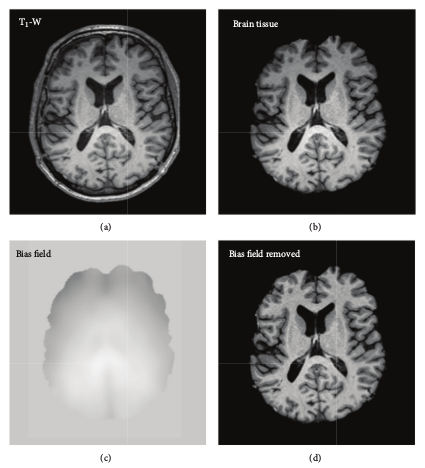
\includegraphics[scale=0.7]{9Preprocessing}\caption{Triangulation for the 15 patterns. \label{fig:Preprocessing}}
\end{figure}

The most important steps are: MRI bias field correction, image registration and brain extraction. 

\textit{Basic}
An image for segmentation can be defined in 2D space (pixels) or in 3D space (voxels). Each image element is specified by its intensity value and coordinates for pixels (i,j) and for voxels (i,j,k). Intensity values are typically represented by a gray value {0, …, 255}. 

The goal of image segmentation is to divide an image into a set of semantically meaningful, homogeneous, and nonoverlapping regions of similar attributes such as intensity, depth, color, or texture. Thesegmentation result is either an image of labels identifying each homogeneous region or a set of contours which describe the region boundaries.

Fundamental components of structural brain MRI analysis include the classification of MRI data into specific tissue types and the identification and description of specific anatomical structures. The problems of segmentation and classification are interlinked because segmentation implies a classification, while a classifier implicitly segments an image. In the case of brain MRI, image elements are typically classified into three main tissue types: white matter (WM), gray matter (GM), and cerebrospinal fluid (CSF) (Fig. \ref{fig:Segment}).

\begin{figure}[H]
\centering{}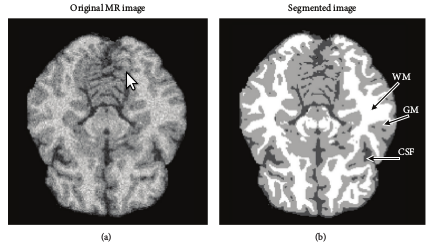
\includegraphics[scale=0.7]{9Segmentation}\caption{Triangulation for the 15 patterns. \label{fig:Segment}}
\end{figure}

One of the most important features for brain MRI segmentation is the intensity of brain tissue. However, intensity-based segmentation algorithms will lead to wrong results when intensity value are corrupted by MRI artifacts. 

\textit{MRI Segmentation Methods}
There is no single method that can be suitable for all images, nor are all methods equally good for a particular type of image. For example, some of the methods use only the gray level histogram, while some integrate spatial image information to be robust for noisy environments. Some methods use probabilistic or fuzzy set theoretic approaches, while some additionally integrate prior knowledge (specific image formation model, e.g., MRI brain atlas) to further improve segmentation performance.
The segmentation methods, with application to brain MRI, may be grouped as follows:
\begin{itemize}
	\item manual segmentation;
	\item intensity-based methods (including thresholding, region growing, classification, and clustering);
	\item atlas-based methods;
	\item surface-based methods (including active contours and surfaces, and multiphase active contours);
	\item hybrid segmentation methods.
\end{itemize}


\hfill\newline
\textbf{List of References}\newline
\cite{09a1} 

\section{Module 9}

Interpolation is a method of constructing new points based on the
existing ones. In other words finding a value of a new point in High
Resolution (HR) image based on points in Low Resolution (LR) pictures.

In classical interpolation techniques pixels in LR data $y$ can be
related to the corresponding $x$ values of HR data: $y_{p}=\frac{1}{N}\sum_{i=1}^{N}x_{i}+n,$
where $y_{p}$ is the pixel of LR image at location $p$, $x_{i}$
is each one of the $N$ High Resolution pixels contained within this
LR pixel and $n$ is some additive noise.

The biggest problem is that to find High Resolution data from the
Low Resolution values. Unfortunately, there is an infinite number
of values that meet that condition. Interpolation methods can be divided
into three basic techniques.

The first group are the most common ones, like linear or spline-based
interpolation. These techniques assume that it is possible to count
the value of a new point by determination some kind of generic function.
The main disadvantage is that they are correct only for images of
homogeneous regions. As is well known, brain consists of grey substance,
white substance and cerebral spinal fluid, so above-mentioned methods
are not appropriate for MRI images interpolation. The second one is
Super Resolution technique. It is commonly used to increase image
resolution on functional MRI (fMRI) and Diffusion Tensor Imaging (DTI).
The method is based on acquisition of multiple Low Resolution (LR)
images of the same object. It is time consuming and not adequate for
clinical applications.

The last but not least method is non-local patch-based technique which
is based on self-similarity of a single image. It is possible to improve
resolution by extracting information from a single image instead of
acquiring several pictures.

The aim of this module is to increase MRI image resolution by upsampling.
The input data is a single 320x240 image. After the processing it
is going to be twice as big. To be more specific 640x480 pixels. The
process can be named as double upsampling.

The first step of the algorithm is to divide every pixel of LR image
into more pixels. Then the patch is designed. It is a rectangle which
will be the area of interest. The pixels that are inside the area
are taken into account during calculation the values of new points.
After that an appropriate estimator is used to correctly calculate
the values of new pixels. Every pixel has to be classified into one
of three groups (grey substance, white substance or cerebral spinal
fluid).

\hfill\newline
\textbf{List of References}\newline
\cite{9art1}

\section{Module 10}

\indent To prepare tree dimension visualization of the cerebral cortex
is used algorithm of marching cubes.\\
 \indent The input data is multiple 2D slices of MR image. The marching
cubes algorithm create a polygonal representation of constant density
surfaces from a 3D array of data. To select the cerebral cortex is
used output data from segmentation made in module 8. The space of
the image is divided into a regular grid of cubes. In each iteration
one cube is considered. At each vertex of cube is determined how the
surface intersects this cube. The density value and compared with
the limit value - surface constant. If the data value is bigger than
suface constant, one is assinged to a cube's vertex. There are 256
combinations of cube orientation relative to the surface, but we can
distinguish 15 basic patterns, that repeat as symmetrical reflections,
produces all possibilities (Fig. \ref{fig:Marching cubes}). If all
values \LyXZeroWidthSpace \LyXZeroWidthSpace are less than the constant
value, then the cube does not form any polygon. Otherwise, the edges
of the polygon are defined (by linear interpolation) at the edges
that intersect the surface. Using central differences, a unit normal
at each cube vertex is calculated and then normal to each trangle
vertex is interpolated. The output of the algorithm is the triangle
vertices and vertex normals.

\begin{figure}[H]
\centering{}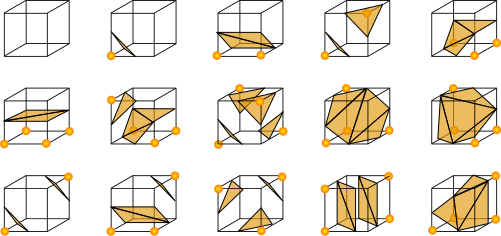
\includegraphics[scale=0.7]{MarchingCubes}\caption{Triangulation for the 15 patterns. \label{fig:Marching cubes}}
\end{figure}

\indent To visualization the model, obtained by marching cubes, the
VTK library is used, which enables building the three-dimension model.
\\
 \indent The second part of this module includes visualization of
the brain's cross-section on arbitrarily defined plane. \\
 \indent

There are three primary imaging planes that are performed in medical
imaging: 
\begin{itemize}
\item axial plane, which is any plane that divides the body into superior
and inferior parts, roughly perpendicular to spine. 
\item sagittal plane, which is any imaginary plane parallel to median plane. 
\item coronal plane, which is any vertical plane that divides the body into
anterior and posterior sections. 
\end{itemize}
The MRI produces two-dimensional images that consist of slices of
brain's and is usually performed in axial plane. To receive images
in the remaining planes, linear interpolation is used

\section{Module 11}

\indent The literature to this module is as useful as nipples on men. Everything is about inventing how to realize point 1. of the list. \\
\indent Oblique Imaging is a technique to create non-perspective projections from 3D or multiple 2D images.\\

\indent In order to create oblique image it is essential to:
\begin{itemize}
\item choose two angles under which the plane will be inclined,
\item create a matrix of points that this plane consists of,
\item from existing points pick those, which will be used in the image,
\item interpolate points that are not existing.
\end{itemize}
\indent Type of interpolation can vary, but in this project interpolation based on mean will be used.
To interpolate one pixel mean of all pixels around him with given proximity is taken.

\begin{figure}[H]
\centering{}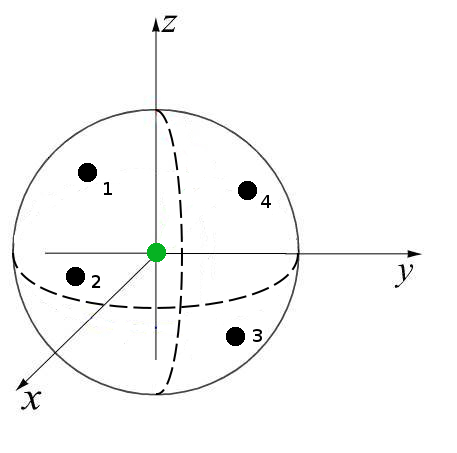
\includegraphics[scale=0.7]{m11_spherexyz}\caption{Visualization of pixels taken to interpolate} \label{fig:m11_spherexyz }
\end{figure}
\chapter{Implementation}

\section{Tools}

\textbf{Python} - The main programming language of this project is Python. The utilized language version is \textbf{Python 3.5.4} (last "bugfix" release of Python 3.5).

\textbf{VTK} - The Visualization Toolkit (VTK) is an open-source software system for 3D computer graphics, modeling, image processing, volume rendering, scientific visualization, and information visualization.
The project uses version \textbf{7.0}, as it is compatible with python 3.5 (compatibility assured by menpo project\footnote{http://www.menpo.org/}).

\textbf{Cython} - Cython is an optimising static compiler for both the Python programming language and the extended Cython programming language. It allows to represent the most computionally complex operations with more efficient code. This project uses version \textbf{0.26.1}.

\textbf{PyQT} - PyQt brings together the Qt C++ cross-platform application framework and the cross-platform interpreted language Python. This project uses its version \textbf{5.6} to create Graphical User Interface (GUI) for the application.

\textbf{Conda} - Conda is an open source package management system and environment management system that runs on Windows, macOS and Linux. Conda quickly installs, runs and updates packages and their dependencies. This project uses \textbf{Anaconda3} distribution to provide standarized enviroment with all of the required packages for our developers.

\section{Module 1}

-code

\section{Module 2}

-code 

\section{Module 3}

-code 

\section{Module 4}

-code 

\section{Module 5}

-code 

\section{Module 6}

-code 

\section{Module 8}

-code 

\section{Module 9}

-code 

\section{Module 10}

-code 

\section{Module 11}

-code

\chapter{Tests}

\section{Module 1}

-module 1 tests 

\section{Module 2}

\section{Module 3}

\section{Module 4}

\section{Module 5}

\section{Module 6}

\section{Module 8}

\section{Module 9}

\section{Module 10}

\section{Module 11}

\section{Application}

-whole app tests

\chapter{Authors}

Authors of this project are students of Biomedical Engineering, AGH
UST, Krakow, Poland. \\
 
\begin{center}
\begin{tabular}{|c|c|}
\hline 
Name  & Role \tabularnewline
\hline 
\hline 
Sylwia Mól  & Project Manager\tabularnewline
\hline 
Jacek Fidos  & Software architect\tabularnewline
\hline 
Maciej Gryczan  & GUI engineer\tabularnewline
\hline 
Adrian Stopiak  & Vizualization engineer \tabularnewline
\hline 
Malwina Molendowska  & 1st module developer \tabularnewline
\hline 
Klaudia Gugulska  & 2nd module developer \tabularnewline
\hline 
Kacper Turek  & 3rd module developer \tabularnewline
\hline 
Magdalena Rychlik  & 4th module developer \tabularnewline
\hline 
Alicja Martinek  & 5th module developer \tabularnewline
\hline 
Mateusz Pabian  & 6th module developer \tabularnewline
\hline 
Anna Grzywa  & 8th module developer \tabularnewline
\hline 
Magdalena Kucharska  & 9th module developer \tabularnewline
\hline 
Eliza Kowalczyk  & 9th module developer \tabularnewline
\hline 
Karolina Gajewska  & 10th module developer \tabularnewline
\hline 
Michał Kotarba  & 11th module developer \tabularnewline
\hline 
\end{tabular}
\par\end{center}

\newpage{}

\listoffigures

\printbibliography

\begin{comment}
 \bibliographystyle{plain}
\bibliography{bibliografia}
 
\end{comment}

\end{document}
